% chercher des documents LaTeX dans styles, corps et bib
\makeatletter\def\input@path{{styles/}{corps/}}\makeatother
\documentclass{rapport}
\usepackage{graphicx}
\usepackage{tikz}
\usetikzlibrary{shapes.geometric, arrows, positioning}
\usetikzlibrary{fit}
\usepackage{subcaption}
\usepackage{placeins}
\usepackage{float}
\usepackage{xcolor}
\usepackage{amsmath}
\usepackage{hyperref}
\usepackage{pgffor}
\usepackage{pgf, pgffor, amsmath}
\usepackage{fancyhdr}
\usepackage{pdfpages}

\usetikzlibrary{positioning, shapes, arrows.meta}
\usepackage{pdflscape}
\usepackage{caption}
\usepackage{geometry}
\usepackage{acronym}
\usepackage{cleveref}
\usepackage{appendix}
\usepackage{tikz}
\usetikzlibrary{calc}
\usepackage{listings}
\usepackage{xcolor}
%\usepackage[linesnumbered,ruled,vlined]{algorithm2e}
%\usepackage[linesnumbered, ruled, vlined]{algorithm2e}
%\usepackage[ruled,vlined]{algorithm2e}
\usepackage[ruled,vlined,linesnumbered]{algorithm2e}
%\usepackage{algorithm}
%\usepackage{algorithmic}


\title{\vspace{1cm} Combination of Stochastic Model Predictive Control and Vision System on a Donkey Car for Circuit Following Task}
\author{Ambre \textsc{Ricouard}\\
  \texttt{ambre.ricouard@ensta-bretagne.org}}
\date{October 1, 2024}
\etablissement{\textsc{Ensta} Bretagne\\2, rue Fran�ois Verny\\
  29806 \textsc{Brest} cedex\\\textsc{France}\\Tel +33 (0)2 98 34 88 00\\ \url{www.ensta-bretagne.fr}}
\logoEcole{\includegraphics[height=4.2cm]{logo_ENSTA_Bretagne_Vertical_CMJN}}

% Insertion de l'image

% M�tadonn�es � inclure dans le pdf
\hypersetup{%
  pdftitle={intern_report},
  pdfauthor={Ambre Ricouard},
  pdfkeywords={internship report},
  bookmarksnumbered,
  pdfstartview={FitH},
  citecolor=blue,
  breaklinks=true
}%

% Cr�er le glossaire
\makeglossaries
% Cr�er l'index
\makeindex

% Redefine \maketitle to include logo
\makeatletter
\renewcommand{\maketitle}{
    \begin{titlepage}
        \centering
        \begin{minipage}{0.35\textwidth}
            \centering
            \includegraphics[width=\textwidth]{logo_ENSTA_Bretagne_Vertical_CMJN}
        \end{minipage}
        \hfill
        \begin{minipage}{0.55\textwidth}
            \centering
            \includegraphics[width=\textwidth]{imgs/tu_wien.jpeg}
        \end{minipage}
        \vspace{1cm} % Ajustez l'espace entre les logos et le titre
        {\Huge \bfseries \@title \par}
        \vspace{0.5cm} % R�duire l'espace entre les lignes du titre
        {\Large \@author \par}
        \vfill
        {\large \@date \par}
        \vfill
        {\large \@etablissement \par}
        \vfill
    \end{titlepage}
}
\makeatother

\pagestyle{fancy}
\fancyhf{}
\fancyhead[L]{\includegraphics[height=1cm]{logo_ENSTA_Bretagne_Vertical_CMJN}}
\fancyhead[R]{\includegraphics[height=1cm]{imgs/tu_wien.jpeg}}
\fancyfoot[C]{\thepage}

\begin{document}

% D�but du pr�ambule
\frontmatter
% Inclure la liste des acronymes
\input{acronymes}
% Cr�er le titre ici
\maketitle 

% Chargement du fichier abstract.tex
\selectlanguage{english}
\section*{\small Abstract}
\small
This project focuses on automating a small-scale model car to navigate a fixed circuit using only a camera for guidance. The objective is for the car to follow a track centered between two guiding lines. The circuit used in reality is also available in simulation, allowing for process validation before testing in a real environment where significant visual noise may be present.

A crucial initial step is to examine the system specifications and camera limitations to anticipate all possible scenarios, thereby ensuring that the developed controllers are robust. Depending on the car's position and orientation relative to the track, it may detect both lines, only one line, or even none. Therefore, the system must be able to handle each of these situations effectively.

The process begins with image processing, where the visible lines are detected to determine the car's orientation and desired future position. With this information in hand, the next step is to address vehicle control. This requires establishing the car's kinematic model, which involves defining a projection frame and understanding how the system inputs relate to the vehicle's kinematics.

Initially, a simple Proportional-Integral-Derivative (\acs{PID}) controller is implemented. While this provides a good starting point, it is inherently limited as it only accounts for past positions. To improve system robustness, a stochastic Model Predictive Control (\acs{MPC}) algorithm is introduced, enabling for the prediction of future trajectories and more effective decision-making.


\section*{\small R\'esum\'e}
Ce projet se concentre sur l'automatisation d'une voiture miniature naviguant sur un circuit fixe, en utilisant une cam\'era comme unique capteur. L'objectif est que la voiture suive une piste d\'elimit\'ee par deux lignes continues. Le circuit r\'eel est \'egalement disponible en simulation, permettant de valider les traitements avant de les tester dans l'environnement r\'eel, o\`u le bruit visuel est significatif.

La premi\`ere \'etape consiste \`a examiner les sp\'ecifications du syst\`eme et les limitations de la cam\'era afin d'anticiper tous les sc\'enarios possibles, assurant ainsi la robustesse des contr\^oleurs d\'evelopp\'es. Selon la position et l'orientation de la voiture par rapport \`a la piste, celle-ci peut d\'etecter les deux lignes, une seule ligne, ou aucune. Le syst\`eme doit donc \^etre capable de g\'erer efficacement chacune de ces situations.

Vient ensuite le traitement des images de la cam\'era pour identifier les lignes visibles, permettant ainsi de d\'eterminer la position et l'orientation futures de la voiture. Avec ces informations, on aborde le contr\^ole du v\'ehicule, ce qui n\'ecessite d'\'etablir le mod\`ele cin\'ematique de la voiture, incluant la d\'efinition d'un rep\`ere de projection et la compr\'ehension de la relation entre les entr\'ees et le mouvement du v\'ehicule.

Initialement, un contr\^oleur Proportionnel-Int\'egral-D\'eriv\'e (\acs{PID}) simple est mis en \oe uvre. Bien que cela constitue un bon point de d\'epart, il pr\'esente des limitations intrins\`eques, car il ne prend en compte que les positions pass\'ees de la voiture. Pour am\'eliorer la robustesse du syst\`eme, un algorithme de contr\^ole pr\'edictif bas\'e sur une commande pr\'edictive (\acs{MPC}) est introduite, permettant de pr\'evoir les trajectoires futures et de prendre des d\'ecisions plus efficaces.



\section*{Keywords}
Autonomous Car, Camera, Image Processing, Line Following, \acs{PID} Control, \acs{MPC} Control.



\section*{Acknowledgements}

I would like to express my deepest gratitude to Alexander Watcher and Gerald Ebmer for their invaluable assistance in helping me initiate this project. Their unwavering support and guidance have been instrumental in my progress, as they were always available to answer my questions and provide clarity. I am also profoundly thankful to my internship supervisor, Minh Nhat Vu, whose supervision and insightful advice have been pivotal to the successful completion of this project. Thank you for your dedicated mentorship and continuous encouragement.

%%% Local Variables: 
%%% mode: latex
%%% TeX-master: "../guide"
%%% End: 


\clearpage

% Table des mati�res
\tableofcontents

\clearpage

% Partie principale
\mainmatter
% Chargement du fichier corps.tex
% fonction pour dessiner la voiture � partir des coordonn�es du point milieu avant
% D�finir la commande drawCar
% Fonction pour dessiner la voiture � partir des coordonn�es du point milieu avant
\newcommand{\drawCar}[9]{
    \def\xFront{#1}
    \def\yFront{#2}
    \def\theta{#3}
    \def\wheelAngle{#4}
    \def\scale{#5}
    \def\drawCarDirection{#6}
    \def\drawWheelDirection{#7}
    \def\xTarget{#8}
    \def\yTarget{#9}
    \def\showTheta{0}  % Fix� � 0 pour simplifier
    \def\showPsi{0}    % Fix� � 0 pour simplifier
    \def\showObj{0}    % Fix� � 0 pour simplifier

    % Dimensions de la voiture et des roues en fonction de l'�chelle
    \def\carLength{4*\scale}
    \def\carWidth{2*\scale}
    \def\wheelLength{1*\scale}
    \def\wheelWidth{0.4*\scale}

    % Ajouter un epsilon pour �viter les divisions par z�ro
    \pgfmathsetmacro{\epsilon}{0.0001}
    \pgfmathsetmacro{\xFrontAdj}{ifthenelse(\xFront==0, \epsilon, \xFront)}
    \pgfmathsetmacro{\yFrontAdj}{ifthenelse(\yFront==0, \epsilon, \yFront)}

    % Calculer le centre de la voiture
    \pgfmathsetmacro{\x}{\xFrontAdj - (\carLength/2) * cos(\theta)}
    \pgfmathsetmacro{\y}{\yFrontAdj - (\carLength/2) * sin(\theta)}

    % Dessiner la voiture (rectangle)
    \begin{scope}[shift={(\x,\y)}, rotate=\theta, scale=\scale];
        \draw[thick] (-\carLength/2, -\carWidth/2) rectangle (\carLength/2, \carWidth/2);

        % Dessiner les roues arri�re (rectangles arrondis, remplis en blanc)
        \filldraw[white, thick, rounded corners=0.1cm]
            (-\carLength/2-\wheelLength/2, -\carWidth/2-\wheelWidth) rectangle (-\carLength/2+\wheelLength/2, -\carWidth/2);
        \draw[thick, rounded corners=0.1cm]
            (-\carLength/2-\wheelLength/2, -\carWidth/2-\wheelWidth) rectangle (-\carLength/2+\wheelLength/2, -\carWidth/2);

        \filldraw[white, thick, rounded corners=0.1cm]
            (-\carLength/2-\wheelLength/2, \carWidth/2) rectangle (-\carLength/2+\wheelLength/2, \carWidth/2+\wheelWidth);
        \draw[thick, rounded corners=0.1cm]
            (-\carLength/2-\wheelLength/2, \carWidth/2) rectangle (-\carLength/2+\wheelLength/2, \carWidth/2+\wheelWidth);

        % Dessiner les roues avant (rectangles arrondis, remplis en blanc avec angle)
        \begin{scope}[shift={(\carLength/2, -\carWidth/2-\wheelWidth/2)}, rotate=\wheelAngle];
            \filldraw[white, thick, rounded corners=0.1cm]
                (-\wheelLength/2, -\wheelWidth/2) rectangle (\wheelLength/2, \wheelWidth/2);
            \draw[thick, rounded corners=0.1cm]
                (-\wheelLength/2, -\wheelWidth/2) rectangle (\wheelLength/2, \wheelWidth/2);
        \end{scope};

        \begin{scope}[shift={(\carLength/2, \carWidth/2+\wheelWidth/2)}, rotate=\wheelAngle];
            \filldraw[white, thick, rounded corners=0.1cm]
                (-\wheelLength/2, -\wheelWidth/2) rectangle (\wheelLength/2, \wheelWidth/2);
            \draw[thick, rounded corners=0.1cm]
                (-\wheelLength/2, -\wheelWidth/2) rectangle (\wheelLength/2, \wheelWidth/2);
        \end{scope};

        % Dessiner la direction de la voiture si l'option est activ�e
        \ifnum\drawCarDirection=1
            \draw[dashed] (0,0) -- (\carLength/2 + 5, 0);
        \fi;

        % Dessiner la direction des roues avant si l'option est activ�e
        \ifnum\drawWheelDirection=1
            \begin{scope}[shift={(\carLength/2, -\carWidth/2-\wheelWidth/2)}, rotate=\wheelAngle];
                \draw[dashed] (0,0) -- (3.5*\wheelLength, 0);
            \end{scope};
        \fi;
    \end{scope};

    \ifnum\showObj=1
        % Dessiner une ligne pointill�e entre (x_d, y_d) et le point milieu avant de la voiture
        \draw[dashed] (\xTarget, \yTarget) -- (\xFront, \yFront-0.3);
        \filldraw[red] (\xFront+0.13,\yFront-0.39) circle (2pt);
    \fi;

    \ifnum\showTheta=1
        % Calculer l'angle entre la direction de la voiture et la ligne pointill�e
        \pgfmathsetmacro{\deltaX}{\xTarget - \xFront}
        \pgfmathsetmacro{\deltaY}{\yTarget - \yFront}
        \pgfmathsetmacro{\angleLine}{atan2(\deltaY, \deltaX)}
        \pgfmathsetmacro{\angleDifference}{\theta - \angleLine}

        % Dessiner une fl�che courbe pour indiquer l'angle
        \draw[->, >=stealth, thick] (\xFront+0.13, \yFront-0.39) +(\theta:1.45) arc (\theta:\angleLine:1.45);

        % Ajouter la lettre grecque \(\theta\) au-dessus de la fl�che courbe
        \node at ($(\xFront,\yFront) + ({(\angleLine+\theta)/2}:1.5)$) {\(\theta\)};
    \fi;

    \ifnum\showPsi=1
        % Dessiner une fl�che courbe pour indiquer l'angle entre la direction de la voiture et la direction des roues avant (\(\psi\))
        \pgfmathsetmacro{\wheelDirection}{\theta + \wheelAngle}
        \draw[->, >=stealth, thick] (\xFront+0.13, \yFront-0.39) +(\theta:1.1) arc (\theta:\wheelDirection:2.8);

        \node at ($(\xFront+0.75,\yFront-0.25) + ({(\angleLine+\wheelDirection)/2}:1.5)$) {\(\psi\)};
    \fi;
}

% D�finir une commande pour extraire les arguments d'une liste
\newcommand{\ntharg}[2]{
    \foreach \n [count=\i] in {#1} {
        \ifnum\i=#2 \relax
            \n
        \fi;
    };
}

% Define the drawVectors function
\newcommand{\drawVectors}[3]{
    % Parameters: x, y, orientation
    \def\x{#1}
    \def\y{#2}
    \def\theta{#3}
    
    % Draw car velocity vector
    \draw[->, thick, red] (\x,\y) -- ++({\theta}:1.5) node[above] {$v$};
    
    % Draw wheel velocity vector
    \pgfmathsetmacro{\wheelAngle}{\theta - 20} % + 20}
    \draw[->, thick, blue] (\x,\y) -- ++({\wheelAngle}:1.0) node[above] {$v_{\text{wheel}}$};
    
    % Draw tangential velocity vector
    \pgfmathsetmacro{\tanAngle}{\theta - 90}
    \draw[->, thick, orange] (\x,\y) -- ++({\tanAngle}:1.0) node[above] {$v_{\text{tan}}$};
    
    % Draw the angle between v_car and v_wheel
    %\pgfmathsetmacro{\psiAngle}{\theta - 10} % Adjust this value to place the label correctly
    %\draw[->, >=stealth, thick] (\x,\y) +(\theta:1.5) arc (\theta:\wheelAngle:1.5);
    %\node at ($(\x,\y) + ({(\theta + \wheelAngle)/2}:1.7)$) {\(\psi\)};
}
\section*{Introduction}

Automating vehicles holds the promise of significantly reducing human error, a major factor in road accidents. According to the World Health Organization, approximately 90 \% of road traffic accidents are attributed to human error \cite{who_road_safety}. By eliminating these errors, autonomous vehicles have the potential to save thousands of lives and reduce severe injuries.

However, ensuring that automated systems are truly effective requires them to be both robust and reliable. Achieving this reliability is a complex challenge due to the diverse and variable environments in which vehicles operate. Road conditions, the behavior of other road users, and weather variations make the task particularly difficult.

Given these challenges, real-world testing of these systems is often costly and risky. To address these issues, researchers are increasingly turning to reduced-scale model cars. These smaller models enable safe and cost-effective experimentation while providing valuable insights into the behavior and performance of autonomous driving technologies (\cite{stocco2022mind}). By using scaled-down versions, we can rigorously test and refine autonomous driving systems in a controlled setting, accelerating their development while managing the financial and safety concerns associated with full-scale testing. \\

The goal of this project is to make an existing reduced-scale model car autonomous, enabling it to navigate a given track using only a camera. The system must be optimized to ensure stability, achieving a smooth trajectory that is resilient to external noise and variations in lighting conditions.

The first step in the process is to thoroughly understand the specific characteristics and limitations of the existing model car system. Once this foundational knowledge is established, the next phase involves processing the camera images to accurately detect the circuit lines. With the track detection in place, a suitable controller must then be designed to effectively manage the car's movements and ensure stable navigation.

In this approach, a \acs{PID} controller will be employed first, followed by a transition to using a \acs{MPC}. Starting with the \acs{PID} controller ensures a simple and straightforward control mechanism. The subsequent implementation of \acs{MPC} will enhance the system's performance by leveraging predictive capabilities and optimization, allowing for more precise, efficient and robust control. This phased approach provides a balance between simplicity and advanced functionality, ultimately improving the overall system performance.





\section{System Overview}
\label{sec:gen}

\subsection{Description of the Car Components}

The model car system consists of several key components that work together to enable autonomous navigation. Figure \ref{tab:components} provides a detailed description of each component and its role in the system. All electronic components are controlled by the onboard Raspberry Pi 4 computer.


\begin{figure}[H]
    \centering
    \includegraphics[width=0.6\textwidth]{imgs/donkey_car.pdf} % R�duit la taille de l'image
    \caption{General view of car.}
    \label{fig:donkey_car}
\end{figure}

\begin{table}[H]
    \centering
    \begin{tabular}{|c|l|}
        \hline
        \textbf{Component} & \textbf{Description} \\
        \hline
        Chassis & The main frame of the car, which supports all other components. \\
        \hline
        Driving motor & Electronic Speed Controller (\acs{ESC}), Rear-Wheel Drive \\
        \hline
        Servo motor & Steering the front wheels with a range of 90� \\
        \hline
        Raspberry Pi 4 & The onboard computer that processes sensor data and controls the car. \\
        \hline
        Pi Camera V2 & Captures visual data of the track for navigation purposes. \\
        \hline
    \end{tabular}
    \caption{Detailed description of the car's components.}
    \label{tab:components}
\end{table}

As indicated in Table \ref{tab:components}, the system's only sensor is the Pi Camera. Thus, image processing is the only means of determining the car's position relative to the track boundaries. Using the onboard camera, the system captures real-time images that are then processed by the Raspberry Pi.

The car is equipped with two types of motors for control: a servo motor and an \acs{ESC}. The servo motor is responsible for angular speed, allowing the front wheels to turn and steer the car. The input command for the servo motor, which determines the steering angle, rannonges from -1 to 1. A value of -1 corresponds to maximum left steering, 0 to a neutral position, and 1 to maximum right steering.

The \acs{ESC} controls the car's linear speed. It also regulates the power sent to the rear wheels, allowing the car to accelerate or decelerate. The input command ranges from 0 to 1, where 0 corresponds to a complete stop and 1 to maximum speed.

These two commands are essential for driving the car, and their combination allows for effective navigation of the track, following the defined trajectory.

The circuit's Command and Control (\acs{C2}) Architecture, as shown in \autoref{sec:c2_architecture}, illustrates the interactions between the car's components and clearly distinguishes the hardware aspects from the observation and control processes.

\subsection{Environment and circuit}
The real circuit is available in simulation, allowing for an initial focus on achieving the objectives in a controlled environment. This helps mitigate environmental noise and facilitates effective validation of image processing and control algorithms before applying them in the real world.

\begin{figure}[H]
    \centering
    \begin{subfigure}[b]{0.45\textwidth}
        \centering
        \includegraphics[width=\textwidth]{imgs/circuit_reel.png}
        \caption{Real Circuit}
        \label{fig:image1}
    \end{subfigure}
    \hfill
    \begin{subfigure}[b]{0.45\textwidth}
        \centering
        \includegraphics[width=\textwidth]{imgs/circuit_simu.png}
        \caption{Simulated Circuit}
        \label{fig:image2}
    \end{subfigure}
    \caption{Circuit the car must follow: (a) Real circuit, (b) Simulated circuit}
    \label{fig:images}
\end{figure}
%\vspace{-1cm}
Figure \ref{fig:images} shows that the track the car needs to follow consists of two straight sections interrupted by two U-turns, bordered by two orange lines. A dashed white line runs down the center, but due to the light gray background, the contrast between the white line and the background is low, as seen in the real circuit image (Figure \ref{fig:image1}). The contrast appears slightly higher in the simulation (Figure \ref{fig:image2}). Additionally, the discontinuity and curvature of the white line make a Canny filter a less optimal choice for detection.

\begin{figure}[H]
    \centering % Centre l'image
    \includegraphics[width=\textwidth]{imgs/hist_camera.png} % Remplacez par le chemin vers votre image
    \caption{Comparison of camera imagery between simulated and real environments} % L�gende de l'image
    \label{fig:mon_image} % �tiquette pour la r�f�rence
\end{figure}

The images and histograms in Figure \ref{fig:mon_image} compare the visual characteristics and pixel intensity distributions of the real and simulated circuits as captured by the robot's camera. The histogram of the real circuit exhibits a smoother distribution with fewer distinct peaks, highlighting the impact of real-world lighting variations and noise. In contrast, the histogram of the simulated circuit features more distinct peaks, indicating controlled and consistent lighting in the virtual environment. To ensure reliable performance in real-world conditions, incorporating filters into the robot's vision system is essential to reduce noise and enhance robustness against lighting variations.

\subsection{Camera}

To establish a reliable and robust controller, it is crucial to understand all possible input data scenarios. This knowledge ensures that the controller is designed to handle all cases effectively, allowing us to anticipate potential issues and implement solutions that enhance its performance and reliability under various conditions.


\begin{longtable}{|l|l|}
\hline
\textbf{Characteristics} & \textbf{Details} \\
\hline
\endfirsthead

\hline
\textbf{Characteristics} & \textbf{Details} \\
\hline
\endhead

\hline
\endfoot

\hline
\endlastfoot

Resolution & 8 Megapixels (3280 x 2464 pixels) \\
\hline
Sensor & Sony IMX219 \\
\hline
Horizontal Field of View (\acs{FOV}) & Approximately 62.2� \\
\hline
Vertical \acs{FOV} & Approximately 48.8� \\
\hline
Focal Length & 3.04 mm \\
\hline
Aperture & f/2.0 \\
\hline
Lens Type & Fixed \\
\hline
Connection Type & MIPI CSI-2 \\
\hline
Image Output Format & RAW \\
\hline
Shutter type & Rolling shutter \\
\hline
Camera Dimensions & Approximately 25 x 24 x 9 mm \\
\hline
Weight & Approximately 3 g \\
\hline
\caption{Technical specifications of the Pi Camera V2 used in the car system (\cite{raspberry_camera}).}
\label{tab:camera_specs}
\end{longtable}

The camera employs rolling shutter technology, which captures images by scanning the sensor line by line, in contrast to global shutter technology, which captures the entire image simultaneously. In scenarios where the model is moving, the rolling shutter method can theoretically introduce distortions, such as skew or wobble, particularly at high speeds due to the sequential nature of image capture. However, for our small-scale model, the operational speed is relatively low, which minimizes the risk of noticeable distortion. The time required to read out the entire sensor is short enough relative to the model's speed, resulting in negligible positional changes during capture. Consequently, experimental tests have shown no significant image distortion under the current operating conditions. Given the controlled environment and the moderate speed of the model, the rolling shutter is sufficient for our application, balancing image quality, cost, and system complexity effectively.

The camera on the car may not always capture both track lines due to the combined effects of its \acs{FOV}, the car's position, and its orientation. With a horizontal \acs{FOV} of 62.2�, as specified in Table \ref{tab:camera_specs}, the camera covers a limited angular range. When the car is centered and aligned on the track, both lines fall within this range, as observed experimentally. However, if the car deviates from the center or is angled, one line may fall outside the \acs{FOV}. This issue is particularly noticeable during turns or when the car is closer to one line.

Given the circuit's U-turns, the focus must be on the car's immediate surroundings without anticipating the turns. Attention should be directed to the area between 3 cm and 10 cm in front of the vehicle, based on on-site measurements. The perceivable width limits for the car are as follows

\[
\text{Horizontal width at 3 cm} = 2 \times (3 \, \text{cm} \times \tan\left(\frac{\text{\acs{FOV}}}{2}\right)) \approx 3.62 \, \text{cm}
\]

\[
\text{Horizontal width at 10 cm} = 2 \times (10 \, \text{cm} \times \tan\left(\frac{\text{\acs{FOV}}}{2}\right)) \approx 12.06 \, \text{cm}
\]

Given that the field of view at 3 cm is relatively narrow, the car's vision is restricted, making it difficult to see both lines during turns or even on straight sections if the system tends to oscillate. This limited visibility emphasizes the importance of focusing on the immediate area directly in front of the vehicle, especially when navigating sharp bends like U-turns.

\begin{figure}[H]
    \centering
    \begin{tikzpicture}[scale=0.8]  % Ajustez l'�chelle selon vos besoins

    % Exemple d'utilisation de la fonction drawCar avec une �chelle de 0.7
    %\drawCar{0}{0}{110}{-20}{0.7}{1}{1}{2}{-2}{1}{1}{0};  % Voiture au centre point milieu avant en th�orie (pas sur) (5,-5), orientation 110�, roues avant � -20�, �chelle 0.7, direction voiture ON, direction roues ON, point cible (2,-2)
    \drawCar{0}{0}{90}{-20}{0.7}{0}{0}{2}{-2}{1}{0}{0}

    % Road boundaries
    \draw[thick, orange] (-2.5, -3) -- (-2.5, 3);
    \draw[thick, orange] (2.5, -3) -- (2.5, 3);

    % Center line
    \draw[dashed, thick, white] (0, -3) -- (0, 3);

    % Axes
    \draw[->] (-3, 0) -- (3, 0) node[right] {};

    % Labels
    \node[below] at (0, 0) {0};
    \node[below] at (-2, 0) {-$d$};
    \node[below] at (2, 0) {$d$};

    % Perpendicular line at d=0
    \draw[dashed, thick] (0, -3) -- (0, 3);

    % Vecteur
    \draw[->, thick] (0,0) -- (1.5,1.5);

    % Angle entre la ligne pointill�e et le vecteur
    \draw[->, >=stealth, thick] (0, 0) +(90:1.2) arc (90:42:1.2);

    % Affichage du symbole theta
    \node at (1, 1.5) {\texttheta};

    \end{tikzpicture}
    \caption{Definition of \(\theta\) and the axis \(d\) with 0 corresponding to the centerline of the circuit, \(-d\) the left line, and \(d\) the right line.}
    \label{fig:car_in_lane}
\end{figure}


Based on Figure \ref{fig:car_in_lane}, let's define \(\theta\) as the orientation angle of the car relative to the track limits  and \(d\) as the distance from the center. With these definitions, the interdependence of \(\theta\) and \(d\) can be studied to understand the specific scenario, whether one or two lines are detected, depending on their variations.

\begin{figure}[H]
    \centering
    \includegraphics[width=\textwidth]{imgs/d_f_theta_3.png} % Remplacez par le chemin de votre image
    \caption{\(\theta = f(d)\) - Visibility of circuit lines as a function of the car's distance from the center and its orientation angle.}
    \label{fig:example_image}
\end{figure}

According to Figure \ref{fig:example_image}, when positioned at the center ($d = 0$), there is a range of approximately $45.84^\circ$ for consistently detecting both lines. This range decreases significantly as $d$ moves from 0 to 20 cm, reducing to around $11.46^\circ$, indicating a decrease of about 75\%.

Therefore, it is crucial to have a controller with minimal oscillation to remain within the detection zone of both lines on the straight portions of the circuit. Otherwise, the system risks constantly switching between detecting one line and the other without ever detecting both simultaneously, which would compromise the controller's robustness. Additionally, it is important to consider scenarios where only one line is detected (e.g., during U-turns) or no lines are detected (e.g., when leaving the circuit).

\section{Image Processing}
\subsection{Two Lines Detected}
The first approach for detecting the circuit lines would be to use a line detection filter such as the one provided by the Canny algorithm. This algorithm is effective at detecting edges by highlighting sharp transitions between different pixel intensities. However, this method has several drawbacks specific to our context. Firstly, the circuit includes U-turns, which complicates the reliable detection of lines because the Canny algorithm might struggle to follow tight curves. Secondly, the drivable surface of the circuit is rectangular, and the algorithm might mistakenly detect the edges of this surface as relevant lines, which would be an error.

To overcome these issues, we will take advantage of the distinct color contrast between the orange lines of the circuit and the light gray background. By applying a color filter, we can effectively isolate the orange lines without being disturbed by the edges of the circuit or the tight turns. This color-based approach is better suited to our specific situation and should provide more reliable results.


\begin{figure}[H]
    \centering
    \begin{tabular}{cc}
        \begin{subfigure}[t]{0.3\textwidth} % R�duisez la largeur � 40%
            \centering
            \includegraphics[width=\textwidth]{imgs/original_image.png}
            \caption{\acs{RGB} original image}
            \label{fig:step1}
        \end{subfigure} &
        \begin{subfigure}[t]{0.3\textwidth} % R�duisez la largeur � 40%
            \centering
            \includegraphics[width=\textwidth]{imgs/hsv_image.png}
            \caption{Conversion in \acs{HSV}}
            \label{fig:step2}
        \end{subfigure} \\
        \begin{subfigure}[t]{0.3\textwidth} % R�duisez la largeur � 40%
            \centering
            \includegraphics[width=\textwidth]{imgs/masked_image.png}
            \caption{Mask filter}
            \label{fig:step3}
        \end{subfigure} &
        \begin{subfigure}[t]{0.3\textwidth} % R�duisez la largeur � 40%
            \centering
            \includegraphics[width=\textwidth]{imgs/blurred_masked_image.png}
            \caption{Blur filter}
            \label{fig:step4}
        \end{subfigure} \\
        \begin{subfigure}[t]{0.3\textwidth} % R�duisez la largeur � 40%
            \centering
            \includegraphics[width=\textwidth]{imgs/dilated_image.png}
            \caption{Dilated image}
            \label{fig:step5}
        \end{subfigure} &
        \begin{subfigure}[t]{0.3\textwidth} % R�duisez la largeur � 40%
            \centering
            \includegraphics[width=\textwidth]{imgs/image_with_contours.png}
            \caption{Contours detected}
            \label{fig:step6}
        \end{subfigure} \\
        \begin{subfigure}[t]{0.4\textwidth} % R�duisez la largeur � 40%
            \centering
            \includegraphics[width=\textwidth]{imgs/final_result.png}
            \caption{Determination of the angle $\theta$}
            \label{fig:step7}
        \end{subfigure} \\
    \end{tabular}
    \caption{Different steps in the image processing pipeline.}
    \label{fig:process_steps}
\end{figure}

Figure \ref{fig:process_steps} provides a detailed, step-by-step visual representation of the image processing workflow. Each step in the figure illustrates a different stage of the process, showing how the image is progressively transformed through various filtering, masking, and contour detection techniques.

The \acs{RGB} (Red, Green, Blue) image (Figure \ref{fig:step1}) is first converted to the \acs{HSV} (Hue, Saturation, Value) color space (Figure \ref{fig:step2}) to facilitate color segmentation. This transformation allows for easier identification and isolation of specific colors within the image. A mask is then applied to isolate the regions containing the orange lines that define the circuit boundaries (Figure \ref{fig:step3}). 

Subsequently, a blur filter is used to reduce noise and smooth out fine details in the Figure \ref{fig:step4}. This step helps in minimizing minor variations and enhancing the prominence of significant features. Following the blurring, the image is dilated to close gaps and unify disjointed regions (Figure \ref{fig:step5}). Even though these processing steps might not appear to dramatically alter the image, they play crucial roles in ensuring the robustness and consistency of the subsequent analysis. 

Contour detection is then performed on the processed image (Figure \ref{fig:step6}). This step identifies the edges of objects within the image, and the two largest contours are retained as the circuit lines. 

For each of these contours, the moment is calculated (blue points on Figure \ref{fig:step7}). The average of these two centroids determines the target point (red point). Finally, $\theta$, defined as the angle between the vertical line from the camera's position (the bottom center of the image) to the target point, is calculated. This angle is crucial for understanding the vehicle's orientation relative to the track.

%\vspace{-2cm}
\subsection{One Line Detected}

\begin{figure}[H]
    \centering
    \hspace{4cm} % Adjust the value as needed
    \includegraphics[scale=0.7]{imgs/diagram_2.png}
    \caption{Decision diagram for determining \texttheta{} based on line and white line detection.}
    \label{fig:diagram}
\end{figure}

The objective of the image processing is to determine the angle \(\theta\). Figure \ref{fig:diagram} illustrates the process for determining this angle based on the configuration. When both lines are detected, \(\theta\) is calculated using two parameters: the vertical axis of the car and the target point. 
In cases where only one line is detected, an additional data point is needed. To acquire this missing data, the algorithm attempts to detect the white dashed line on image \ref{fig:step2_1} (Figure \ref{fig:white_process_steps}). This involves additional processing steps similar to the previous ones, including masking (\ref{fig:step2_2}), blurring (\ref{fig:step2_3}), and dilation (\ref{fig:step2_3}). The white contours of the dashed line are then used to reconstruct the median white line through linear regression (\ref{fig:step2_4}). The second point is then determined by selecting the point on the line that has the same ordinate as the centroid of the detected contour. 
If case the white line is poorly detected, the algorithm defaults to using the white line detected in the previous frame; if this is not available, it uses the midpoint of the image's width.
If the car deviates and leaves the circuit to the extent that it no longer detects any lines, one solution is to retain the last value of \(\theta\) and increment it slightly to allow the car to find its way back. However, given the narrowness of the circuit, two scenarios are common: either the car takes a considerable amount of time to recalibrate and regain its trajectory, or it has already collided with an obstacle, such as a wall or another surrounding object.



\begin{figure}[H]
    \centering
    \begin{tabular}{cc}
        \begin{subfigure}[t]{0.3\textwidth} % R�duisez la largeur � 40%
            \centering
            \includegraphics[width=\textwidth]{imgs/one_line_original_image.jpg}
            \caption{\acs{RGB} original image}
            \label{fig:step2_1}
        \end{subfigure} &
        \begin{subfigure}[t]{0.3\textwidth} % R�duisez la largeur � 40%
            \centering
            \includegraphics[width=\textwidth]{imgs/white_lines_masked_image_lower_half.png}
            \caption{Mask filter}
            \label{fig:step2_2}
        \end{subfigure} \\
        \begin{subfigure}[t]{0.3\textwidth} % R�duisez la largeur � 40%
            \centering
            \includegraphics[width=\textwidth]{imgs/white_lines_blurred_masked_image_lower_half.png}
            \caption{Blur filter}
            \label{fig:step2_3}
        \end{subfigure} &
        \begin{subfigure}[t]{0.3\textwidth} % R�duisez la largeur � 40%
            \centering
            \includegraphics[width=\textwidth]{imgs/white_lines_dilated_image_lower_half.png}
            \caption{Dilated image}
            \label{fig:step2_5}
        \end{subfigure} \\
        \begin{subfigure}[t]{0.3\textwidth} % R�duisez la largeur � 40%
            \centering
            \includegraphics[width=\textwidth]{imgs/image_with_white_line.png}
            \caption{Linear regression of white contours.}
            \label{fig:step2_6}
        \end{subfigure} &
        \begin{subfigure}[t]{0.4\textwidth} % R�duisez la largeur � 40%
            \centering
            \includegraphics[width=\textwidth]{imgs/final_result_white.png}
            \caption{Determination of the angle $\theta$}
            \label{fig:step2_7}
        \end{subfigure} \\
    \end{tabular}
    \caption{Different steps in the image processing pipeline.}
    \label{fig:white_process_steps}
\end{figure}



\section{Kinematics Model}
%\vspace{-0.5cm}
To determine the kinematic model of the system, it is essential to understand the roles of the throttle input \(v\) and the steering angle \(\psi\). Unlike differential drive robots, cars have four wheels, with the two front wheels dedicated to steering and the two rear wheels to propulsion. We will examine how these inputs influence the overall movement of the vehicle.

\subsection{Rear Wheels Analysis and Throttle}

%\vspace{-1cm}

\begin{figure}[H]  % 'htbp' pour "here", "top", "bottom", "page" en options de placement
\centering  % Pour centrer le sch�ma sur la page
\begin{tikzpicture}[scale=0.5]  % R�duction de la taille du sch�ma via l'option de mise � l'�chelle
    % Param�tres configurables
    \def\carLength{3.0}   % Longueur de la voiture
    \def\carWidth{2.0}    % Largeur de l'essieu (distance entre les roues d'un m�me essieu)
    \def\wheelWidth{0.4}  % �paisseur des roues
    \def\wheelDiameter{0.6} % Diam�tre des roues
    \def\innerCircleR{5}  % Rayon du cercle int�rieur de rotation pour les roues arri�re
    \def\wheelAngle{20}   % Angle des roues avant pour tourner � gauche

    % Tracer les cercles de rotation
    \draw[dashed] (0, 0) circle (\innerCircleR);
    \draw[dashed] (0, 0) circle (\innerCircleR + \carWidth);

    % Position de la voiture � la p�riph�rie droite du cercle
    \pgfmathsetmacro{\carPosX}{\innerCircleR + \wheelDiameter/2 + 0.5} % D�calage suppl�mentaire de 0.5 vers la droite
    \pgfmathsetmacro{\carPosY}{0}

    % Dessiner la voiture
    % Corps de la voiture
    \draw[thick] (\carPosX, \carPosY - \carLength/2) -- (\carPosX, \carPosY + \carLength/2);

    % Essieu arri�re et roues arri�re
    \draw[thick] (\carPosX - \carWidth/2, \carPosY - \carLength/2) -- (\carPosX + \carWidth/2, \carPosY - \carLength/2);
    \foreach \x in {-1,1} {
        \draw[thick] (\carPosX + \x*\carWidth/2, \carPosY - \carLength/2 - \wheelDiameter/2) rectangle (\carPosX + \x*\carWidth/2, \carPosY - \carLength/2 + \wheelDiameter/2);
    }

    % Essieu avant et roues avant
    \draw[thick] (\carPosX - \carWidth/2, \carPosY + \carLength/2) -- (\carPosX + \carWidth/2, \carPosY + \carLength/2);
    \foreach \x in {-1,1} {
        \begin{scope}[shift={(\carPosX + \x*\carWidth/2, \carPosY + \carLength/2)}, rotate around={\wheelAngle:(0,0)}]
            \draw[thick] (-\wheelWidth/2, -\wheelDiameter/2) rectangle (\wheelWidth/2, \wheelDiameter/2);
        \end{scope}
    }

    % Vecteur vitesse
    \draw[thick, red, -latex] (\carPosX, \carPosY - \carLength/2) -- ++(0,1.5) node[right] {v};

    % Centre de rotation
    \filldraw[red] (0, 0) circle (2pt);
    \node[below] at (0, -0.5) {Center of Rotation};

\end{tikzpicture}
\caption{Diagram illustrating the kinematics of the rear wheels during a turn with throttle engagement.}
\label{fig:rear_wheels_analysis}
\end{figure}

%\vspace{-1cm}
When the vehicle turns, each wheel follows a circular path around a center of rotation (Figure \ref{fig:rear_wheels_analysis}). Since the rear wheels are mounted on the same axle, they share identical movement characteristics relative to this center. The rear axle aligns with the radii of these concentric circles. Consequently, the velocity of each rear wheel can be represented as a vector originating from the center of the axle and directed perpendicular to it.

\subsection{Front Wheel Analysis and Steering Angles}

\begin{figure}[H]  % 'htbp' pour "here", "top", "bottom", "page" en options de placement
\centering  % Pour centrer le sch�ma sur la page
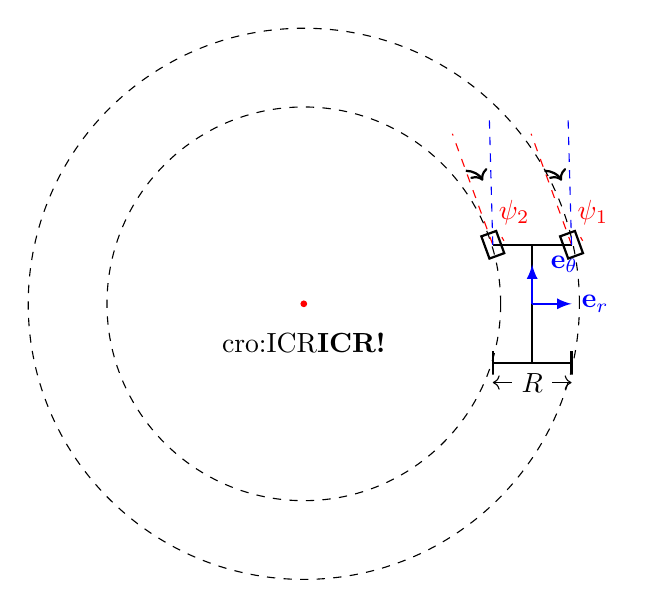
\begin{tikzpicture}[scale=0.5]  % R�duction de la taille du sch�ma via l'option de mise � l'�chelle
    % Param�tres configurables
    \def\carLength{3.0}   % Longueur de la voiture
    \def\carWidth{2.0}    % Largeur de l'essieu (distance entre les roues d'un m�me essieu)
    \def\wheelWidth{0.4}  % �paisseur des roues
    \def\wheelDiameter{0.6} % Diam�tre des roues
    \def\innerCircleR{5}  % Rayon du cercle int�rieur de rotation pour les roues arri�re
    \def\wheelAngle{20}   % Angle des roues avant pour tourner � gauche

    % Tracer les cercles de rotation
    \draw[dashed] (0, 0) circle (\innerCircleR);
    \draw[dashed] (0, 0) circle (\innerCircleR + \carWidth);

    % Position de la voiture � la p�riph�rie droite du cercle
    \pgfmathsetmacro{\carPosX}{\innerCircleR + \wheelDiameter/2 + 0.5} % D�calage suppl�mentaire de 0.5 vers la droite
    \pgfmathsetmacro{\carPosY}{0}

    % Dessiner la voiture
    % Corps de la voiture
    \draw[thick] (\carPosX, \carPosY - \carLength/2) -- (\carPosX, \carPosY + \carLength/2);

    % Lignes de base en bleu
    \draw[thick, blue, -latex] (\carPosX, \carPosY) -- ++(1, 0) node[right] {$\mathbf{e}_r$};
    \draw[thick, blue, -latex] (\carPosX, \carPosY) -- ++(0, 1) node[right=3pt] {$\mathbf{e}_{\theta}$};

    % Essieu arri�re et roues arri�re
    \draw[thick] (\carPosX - \carWidth/2, \carPosY - \carLength/2) -- (\carPosX + \carWidth/2, \carPosY - \carLength/2);
    \foreach \x in {-1,1} {
        \draw[thick] (\carPosX + \x*\carWidth/2, \carPosY - \carLength/2 - \wheelDiameter/2) rectangle (\carPosX + \x*\carWidth/2, \carPosY - \carLength/2 + \wheelDiameter/2);
    }

    % Essieu avant et roues avant avec angles
    \draw[thick] (\carPosX - \carWidth/2, \carPosY + \carLength/2) -- (\carPosX + \carWidth/2, \carPosY + \carLength/2);
    \foreach \x/\label in {-1/2,1/1} {
        \begin{scope}[shift={(\carPosX + \x*\carWidth/2, \carPosY + \carLength/2)}, rotate around={\wheelAngle:(0,0)}]
            \draw[thick] (-\wheelWidth/2, -\wheelDiameter/2) rectangle (\wheelWidth/2, \wheelDiameter/2);
            \draw[dashed, red] (0,0) -- (0,3); % Prolongation horizontale correctement orient�e
            \draw[dashed, blue] (0,0) -- (1,3); % Prolongation de la roue, tourn�e de 90 degr�s vers la droite
            
            % Angle psi
            \draw[red] (0.3,0) arc[start angle=0, end angle=\wheelAngle, radius=0.3];
            \node[red] at ($(0.3,0.5) + (\wheelAngle/2:0.5)$) {$\psi_{\label}$};
            
            % Fl�che en arc de cercle des pointill�s rouges aux pointill�s bleus
            \draw[->, thick] (0, 2) arc[start angle=70, end angle=10, radius=0.5];
        \end{scope}
    }

    % Centre de rotation
    \filldraw[red] (0, 0) circle (2pt);
    \node[below] at (0, -0.5) {\acs{ICR}};
    
    % Indiquer la taille des essieux
    \draw[<->] (\carPosX - \carWidth/2, \carPosY - \carLength/2 - 0.5) -- (\carPosX + \carWidth/2, \carPosY - \carLength/2 - 0.5) node[midway, fill=white] {$R$};

\end{tikzpicture}
\caption{Diagram illustrating the orientations of the front wheels in a polar system.}
\label{fig:front_wheels_analysis}
\end{figure}


The polar coordinate system is centered at the front axle of the vehicle (shifted in Figure \ref{fig:front_wheels_analysis} for clarity). Thus,
the velocities are \(\dot{r} \mathbf{e}_{r} + (r - \frac{R}{2}) \dot{\psi}_1 \mathbf{e}_{\theta}\) for the inner wheel and \(\dot{r} \mathbf{e}_{r} + (r + \frac{R}{2}) \dot{\psi}_2 \mathbf{e}_{\theta}\) for the outer wheel.

To avoid slipping while turning, the front wheels must be tangent to concentric circles centered at a common point, known as the Instantaneous Center of Rotation (\acs{ICR}). Thus, the angular velocities \(\dot{\psi}_1\) and \(\dot{\psi}_2\) must satisfy:
\[
(r - \frac{R}{2}) \dot{\psi}_1 = (r + \frac{R}{2}) \dot{\psi}_2
\]

This equation shows that the inner wheel must turn at a sharper angle than the outer wheel. This configuration allows the car to turn smoothly along a defined circular path without tire slip.

According to \cite{liu2023car} the difference in front angles is known as the Ackermann angle. This can be more easily modeled by introducing a virtual central wheel, positioned between the two front wheels.


\begin{figure}[H]
    \centering
    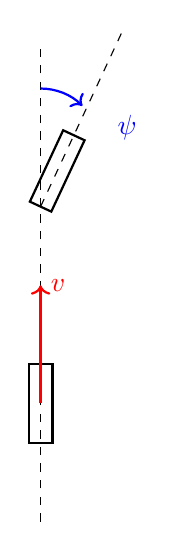
\begin{tikzpicture}[scale=1]

        % Draw rear car (at the bottom)
        \draw[thick] (-0.15, 0) rectangle (0.15, 1); % Reduced height of the car
        \draw[dashed] (0, -1) -- (0, 5); % Less extended centerline

        % Velocity vector
        \draw[->, thick, red] (0, 0.5) -- ++(0, 1.5) node[right] {\(v\)};

        % Draw front car (at the top, very close to rear car)
        \begin{scope}[shift={(0, 3)}, rotate=-25] % Rotate the car for the steering angle towards the left
            \draw[thick] (-0.15, 0) rectangle (0.15, 1); % Reduced height of the car
            \draw[dashed] (0, 0) -- (0, 2.5); % Centerline of the car
        \end{scope}

        % Draw the steering angle arrow and label (between vertical and car's line)
        \draw[->, thick, blue] (0, 4.5) arc[start angle=90, end angle=45, radius=0.75];
        \node[blue] at (1.1, 4) {\(\psi\)};

    \end{tikzpicture}
    \caption{Diagram illustrating the kinematics used in our model.}
    \label{fig:ackerman_diagram}
\end{figure}


The commands for speed and steering angle are now clearly defined with respect to the car (Figure \ref{fig:ackerman_diagram}). Thus, it is now possible to fully determine the kinematic model of the system. 

Subsequently, the car will be illustrated with four wheels for better understanding, but the modeling will remain as shown in Figure \ref{fig:ackerman_diagram}.

\subsection{System Modeling}

The control of the car is solely based on images from the camera, whose position \((x, y)\) corresponds to the middle of the front axle. The angle \(\psi\) represents the steering of the front wheels, while \(\theta\) measures the angle between the car's chassis and the target point \((x_d, y_d)\). The distance \(r\) is defined as the separation between the target point and the car's current position.


\begin{figure}[H]
    \centering
\begin{tikzpicture}[scale=1] % Appliquer un facteur d'�chelle global
  
    % Exemple d'utilisation de la fonction drawCar avec une �chelle de 0.7
    \drawCar{5}{-5}{110}{-20}{0.7}{0}{0}{2}{-2}{1}{0}{0}  % Voiture au centre point milieu avant en th�orie (pas sur) (5,-5), orientation 110�, roues avant � -20�, �chelle 0.7, direction voiture ON, direction roues ON, point cible (2,-2)
	\drawVectors{5.1}{-5.45}{110}
 	
    \end{tikzpicture}
    \caption{The car with its corresponding speed vectors.}
    \label{fig:car_with_legend}
\end{figure}

%\caption{Schematic diagram showing the orientation and velocities of a car's front wheels relative to its chassis.}

Let L be the wheelbase. The lever arm equation is therefore given by
\[
L \cdot \dot{\theta} = v_{\text{tan}} \text{,}
\]
knowing that, according to Figure \ref{fig:car_with_legend},
\[
\left\{
\begin{array}{l}
v_{\text{wheel}} \cos(\psi) = v \\
v_{\text{wheel}} \sin(\psi) = v_{\text{tan}}
\end{array}
\right.
\]
Thus,
\[
v \cdot \tan(\psi) = v_{\text{tan}} \text{.}
\]

Therefore, 
\[
\dot{\theta} = \frac{v \cdot \tan(\psi)}{L} \text{.}
\]

Given that $\psi$ belongs to the interval $[-1, 1]$ (the control limits), we perform a first-order Taylor expansion around $\psi \approx 0$

\[
\dot{\theta} \approx \frac{v \cdot \psi}{L} \text{.}
\]

% fonction pour dessiner la voiture � partir des coordonn�es du point milieu avant
\newcommand{\drawCarSys}[9]{
    \def\xFront{#1}
    \def\yFront{#2}
    \def\theta{#3}
    \def\wheelAngle{#4}
    \def\scale{#5}
    \def\drawCarDirection{#6}
    \def\drawWheelDirection{#7}
    \def\xTarget{#8}
    \def\yTarget{#9}
   
    % Dimensions de la voiture et des roues en fonction de l'�chelle
    \def\carLength{4*\scale}
    \def\carWidth{2*\scale}
    \def\wheelLength{1*\scale}
    \def\wheelWidth{0.4*\scale}
   
    % Calculer le centre de la voiture
    \pgfmathsetmacro{\x}{\xFront - (\carLength/2) * cos(\theta)}
    \pgfmathsetmacro{\y}{\yFront - (\carLength/2) * sin(\theta)}
   
    % Dessiner la voiture (rectangle)
    \begin{scope}[shift={(\x,\y)}, rotate=\theta, scale=\scale]
        \draw[thick] (-\carLength/2, -\carWidth/2) rectangle (\carLength/2, \carWidth/2);
       
        % Dessiner les roues arri�re (rectangles arrondis, remplis en blanc)
        \filldraw[white, thick, rounded corners=0.1cm]
            (-\carLength/2-\wheelLength/2, -\carWidth/2-\wheelWidth) rectangle (-\carLength/2+\wheelLength/2, -\carWidth/2);
        \draw[thick, rounded corners=0.1cm]
            (-\carLength/2-\wheelLength/2, -\carWidth/2-\wheelWidth) rectangle (-\carLength/2+\wheelLength/2, -\carWidth/2);
 
        \filldraw[white, thick, rounded corners=0.1cm]
            (-\carLength/2-\wheelLength/2, \carWidth/2) rectangle (-\carLength/2+\wheelLength/2, \carWidth/2+\wheelWidth);
        \draw[thick, rounded corners=0.1cm]
            (-\carLength/2-\wheelLength/2, \carWidth/2) rectangle (-\carLength/2+\wheelLength/2, \carWidth/2+\wheelWidth);
       
        % Dessiner les roues avant (rectangles arrondis, remplis en blanc avec angle)
        \begin{scope}[shift={(\carLength/2, -\carWidth/2-\wheelWidth/2)}, rotate=\wheelAngle]
            \filldraw[white, thick, rounded corners=0.1cm]
                (-\wheelLength/2, -\wheelWidth/2) rectangle (\wheelLength/2, \wheelWidth/2);
            \draw[thick, rounded corners=0.1cm]
                (-\wheelLength/2, -\wheelWidth/2) rectangle (\wheelLength/2, \wheelWidth/2);
        \end{scope}
 
        \begin{scope}[shift={(\carLength/2, \carWidth/2+\wheelWidth/2)}, rotate=\wheelAngle]
            \filldraw[white, thick, rounded corners=0.1cm]
                (-\wheelLength/2, -\wheelWidth/2) rectangle (\wheelLength/2, \wheelWidth/2);
            \draw[thick, rounded corners=0.1cm]
                (-\wheelLength/2, -\wheelWidth/2) rectangle (\wheelLength/2, \wheelWidth/2);
        \end{scope}
       
        % Dessiner la direction de la voiture si l'option est activ�e
        \ifnum\drawCarDirection=1
            \draw[dashed] (0,0) -- (\carLength/2 + 5, 0);
        \fi
       
        % Dessiner la direction des roues avant si l'option est activ�e
        \ifnum\drawWheelDirection=1
            \begin{scope}[shift={(\carLength/2, -\carWidth/2-\wheelWidth/2)}, rotate=\wheelAngle]
                \draw[dashed] (0,0) -- (3.5*\wheelLength, 0);
            \end{scope}
        \fi
    \end{scope}
 
    % Dessiner une ligne pointill�e entre (x_d, y_d) et le point milieu avant de la voiture
    \draw[dashed] (\xTarget, \yTarget) -- (\xFront, \yFront-0.3);
 
    \filldraw[red] (\xFront+0.13,\yFront-0.39) circle (2pt);
    % Calculer l'angle entre la direction de la voiture et la ligne pointill�e
    \pgfmathsetmacro{\deltaX}{\xTarget - \xFront}
    \pgfmathsetmacro{\deltaY}{\yTarget - \yFront}
    \pgfmathsetmacro{\angleLine}{atan2(\deltaY, \deltaX)}
    \pgfmathsetmacro{\angleDifference}{\theta - \angleLine}
 
    % Dessiner une fl�che courbe pour indiquer l'angle
    \draw[->, >=stealth, thick] (\xFront+0.13, \yFront-0.39) +(\theta:1.45) arc (\theta:\angleLine:1.45);
 
    % Ajouter la lettre grecque ? au-dessus de la fl�che courbe
 
    \node at ($(\xFront,\yFront) + ({(\angleLine+\theta)/2}:1.5)$) {\texttheta};
 
    % Dessiner une fl�che courbe pour indiquer l'angle entre la direction de la voiture et la direction des roues avant (psi)
    \pgfmathsetmacro{\wheelDirection}{\theta + \wheelAngle}
    \draw[->, >=stealth, thick] (\xFront+0.13, \yFront-0.39) +(\theta:1.1) arc (\theta:\wheelDirection:2.8);
 
    \node at ($(\xFront+0.75,\yFront-0.25) + ({(\angleLine+\wheelDirection)/2}:1.5)$) {\(\psi\)};
 
 
}

\begin{figure}[H]
    \centering
    \begin{tikzpicture}[scale=1] % Appliquer un facteur d'�chelle global

        % Dessiner le rep�re
        \draw[->] (-1,0) -- (9,0) node[right] {$x$};
        \draw[->] (0,1) -- (0,-9) node[below] {$y$};

        \draw [dashed] (2,-2) -- (2,0) node[above] {$x_d$};
        \draw [dashed] (2,-2) -- (0,-2) node[left] {$y_d$};

        % Ajouter un point � (2, -2)
        \filldraw[red] (2,-2) circle (2pt);

        % Exemple d'utilisation de la fonction drawCar avec une �chelle de 0.7
        \drawCarSys{5}{-5}{110}{-20}{0.7}{1}{1}{2}{-2}{1}{1}{1}  % Voiture au centre point milieu avant en th�orie (pas sur) (5,-5), orientation 110�, roues avant � -20�, �chelle 0.7, direction voiture ON, direction roues ON, point cible (2,-2)

    \end{tikzpicture}
    
    \caption{Schematic representation of the problem in a Cartesian coordinate system: definition of the target point (xd, yd) and the angles $\theta$ and $\psi$.}
    \label{fig:car_projection}
\end{figure}


Since the target point is to the left of the car, the angle $\theta$ is defined as negative (\ref{fig:car_projection}). Thus, the coordinates \((x, y)\) (represented by the red point on the car) are given by
\[
\left\{
\begin{array}{l}
x = - r \sin(\theta) + x_d\\
y = r \cos(\theta) + y_d
\end{array}
\right.
\]
with:
\[
r = \sqrt{(x - x_d)^2 + (y - y_d)^2}
\]

\begin{figure}[H]
    \centering
    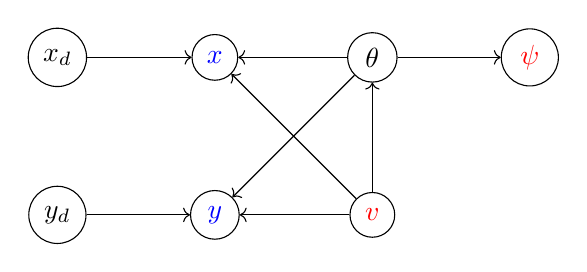
\begin{tikzpicture}[node distance=2cm, auto]
        % Nodes
        \node (x) [draw, circle, text=blue] {$x$};
        \node (y) [below of=x, draw, circle, text=blue] {$y$};
        \node (xd) [left of=x, draw, circle] {$x_d$};
        \node (yd) [left of=y, draw, circle] {$y_d$};
        \node (v) [right of=y, draw, circle, text=red] {$v$};
        \node (theta) [right of=x, draw, circle] {$\theta$};
        \node (psi) [right of=theta, draw, circle, text=red] {$\psi$};

        % Arrows
        \draw[->] (xd) -- (x);
        \draw[->] (yd) -- (y);

        \draw[->] (v) -- (x);
        \draw[->] (v) -- (y);
        \draw[->] (v) -- (theta);

        \draw[->] (theta) -- (x);
        \draw[->] (theta) -- (psi);
        \draw[->] (theta) -- (y);

    \end{tikzpicture}
    \caption{Dependency diagram of state variables (in blue) and commands (in red).}
    \label{fig:bubles}
\end{figure}

The diagram of dependencies (Figure \ref{fig:bubles}) demonstrates that x and y are directely linked to \(v\) and indirectely linked to \(\psi\).

The delay matrix is therefore:
\[
R = \begin{bmatrix}
    1 & 1 \\
    2 & 2
\end{bmatrix}
\]

The minimum coefficients of each row in \( R \) appear in both columns. Therefore, the system is controllable.

\section{Controller}
\subsection{\ac{PID} Controller}

Let's start with a \acs{PID} controller, a logical first step in managing the vehicle's dynamics. Its simplicity and proven effectiveness make it an ideal choice for initial testing and fine-tuning before moving on to more advanced control strategies.
The \acs{PID} controller, by adjusting the proportional, integral, and derivative terms, offers a well-balanced approach to handling errors in real-time. This enables precise control over the car's speed and steering. \\

The structure of the delay matrix \( R \) indicates that some state variables have second-order delays, requiring double differentiation to accurately express \( \begin{pmatrix} x \\ y \end{pmatrix} \) in terms of the inputs \( v \) and \( \psi \).

The derivatives of \( \{x, y\} \) are
\[
\left\{
\begin{array}{l}
\dot{x} = -\dot{r} \sin(\theta) - r \dot{\theta} \cos(\theta) + \dot{x}_d \\
\dot{y} = \dot{r} \cos(\theta) - r \dot{\theta} \sin(\theta) + \dot{y}_d
\end{array}
\right.
\]

Using the first-order approximation for \(\dot{\theta}\),
\[
\left\{
\begin{array}{l}
\dot{x} = -v \sin(\theta) - \frac{r v \psi}{L} \cos(\theta) + \dot{x}_d \\
\dot{y} = v \cos(\theta) - \frac{r v \psi}{L} \sin(\theta) + \dot{y}_d
\end{array}
\right.
\]

Therefore,
\[
\left\{
\begin{array}{l}
\ddot{x} = -\dot{v} \sin(\theta) - v \dot{\theta} \cos(\theta) - \frac{1}{L} [\dot{r} v \psi \cos(\theta) + r \dot{v} \psi \cos(\theta) + r v \dot{\psi} \cos(\theta) - r v \psi \dot{\theta} \sin(\theta)] + \ddot{x}_d \\
\ddot{y} = \dot{v} \cos(\theta) - v \dot{\theta} \sin(\theta) - \frac{1}{L} [\dot{r} v \psi \sin(\theta) + r \dot{v} \psi \sin(\theta) + r v \dot{\psi} \sin(\theta) + r v \psi \dot{\theta} \cos(\theta)] + \ddot{y}_d
\end{array}
\right.
\]

Considering the second-order approximation where \( \dot{v} \cdot \psi = 0\) (implying that the speed varies little and \(\psi\) is small), the second derivatives $\begin{pmatrix} \ddot{x} \\ \ddot{y} \end{pmatrix}$ can be expressed in terms of matrices and vectors as follows,

\[
\begin{pmatrix}
\ddot{x} \\
\ddot{y}
\end{pmatrix}
=
\underbrace{\begin{pmatrix}
-\sin(\theta) & -\frac{r v}{L} \cos(\theta) \\
\cos(\theta) & -\frac{r v}{L} \sin(\theta)
\end{pmatrix}}_A \cdot \underbrace{\begin{pmatrix}
\dot{v} \\
\dot{\psi}
\end{pmatrix}}_U
+
\underbrace{\begin{pmatrix}
\frac{-2 v^2 \psi \cos(\theta)}{L} + \frac{r v^2 \psi^2 \sin^2(\theta)}{2} + \ddot{x}_d \\
\frac{-2 v^2 \psi \sin(\theta)}{L} - \frac{r v^2 \psi^2 \cos^2(\theta)}{2} + \ddot{y}_d
\end{pmatrix}}_B
\]

Thus, let's consider the following \acs{PID}-based control with feedback linearization,
\begin{align*}
    U &= A^{-1}(V - B) \\
    V &= \ddot{X} = k_i(W - X) + k_p(\dot{W} - \dot{X}) + k_d \ddot{W}
\end{align*}
where \( W = \begin{pmatrix} x_d \\ y_d \end{pmatrix} \) and \( k_i \), \( k_p \), and \( k_d \) are the integral, proportional, and derivative gain matrices \\

This controller is implemented in Python and tested within the simulation environment, with the implementation details provided in Algorithm~\ref{alg:pid_control}.

\begin{figure}[H]
    \centering
    \includegraphics[width=1\textwidth]{imgs/theta_t.png} % R�duit la taille de l'image
    \caption{Evolution of $\theta$ over time.}
    \label{fig:theta}
\end{figure}

The desired position for the car is to always have its target point directly in front of the camera, which means that \(\theta\) should ideally be close to 0. However, if \(\theta\) were constantly at 0, the car would follow a straight path, which isn't feasible given the circuit's curves. As a result, \(\theta\) will inevitably deviate from 0 when navigating turns, but the goal is to keep these deviations as small as possible.

It's important to note that the controller is not 100\% robust. There are instances where the car deviates so far from the intended trajectory that it struggles to return to it. To mitigate this, the steering is limited between -0.8 and 0.8, and the speed is capped at 0.02 (Figure \ref{fig:theta}). These constraints are set to reduce oscillations and give the controller enough time to allow the system to converge back to the desired path. Even with these adjustments, while the car usually manages to complete at least one full lap, it can still deviate from its trajectory afterward.

\begin{figure}[H]
    \centering
    \includegraphics[width=1\textwidth]{imgs/new_new_st_t.png} % R�duit la taille de l'image
    \caption{Evolution of steering and throttle over time.}
    \label{fig:s_t}
\end{figure}

The curved and straight segments in the graphical evolution of the steering (Figure \ref{fig:s_t}) can be readily distinguished: rapid and large oscillations correspond to the straight segments, while the segments that exhibit nearly constant behavior indicate the curves. This pattern can also be observed, though less distinctly, in the graph presented in Figure \ref{fig:theta}. The system exhibits significant oscillatory behavior on straight sections of the path, leading to instability as speed increases. Consequently, when the speed becomes too high, the system diverges entirely and loses the track, especially given the tight and short nature of the circuit.

The error graph (Figure \ref{fig:error}) suggests that the controller might be overreacting to small deviations, possibly due to overly aggressive gain settings, particularly for the proportional term. This overreaction leads to oscillations in the system rather than allowing it to smoothly converge to the desired state. However, when the proportional gain is reduced, the system fails to complete even a single lap before diverging. 
Additionally, while the system appears to be diverging based on the error graph, this is not always the case in the simulation. It's important to consider the scale of the errors, which are measured in pixels (elements of the image's numpy array). An error range of 20 pixels, therefore, does not necessarily indicate that the system is completely diverging.

While \acs{PID} controllers are well-suited for point tracking, they often struggle with dynamic trajectories, particularly when the trajectory is unknown and evolves in real-time, frame by frame and point by point. As the target changes, the system oscillates in its attempt to stabilize, only to be disrupted by further trajectory adjustments. This continuous need for adaptation can result in persistent oscillations and a tendency to diverge. To address these challenges, we turn to \acs{MPC}, which is specifically designed to handle such dynamic environments more effectively by anticipating future trajectory changes and optimizing control actions accordingly.


\begin{figure}[H]
    \centering
    \includegraphics[width=1\textwidth]{imgs/error.png} % R�duit la taille de l'image
    \caption{Horizontal error over time.}
    \label{fig:error}
\end{figure}

\subsection{\ac{MPC}}

\acs{MPC} is a sophisticated control strategy that optimizes a system's trajectory over a specified time horizon by predicting its future states. This prediction is crucial for achieving optimal control performance, especially in scenarios that demand precise maneuvering. Therefore, accurately knowing the near-future trajectory is essential.

In our case, the only sensor available is a camera. Therefore, the trajectory prediction capability is constrained by the camera's limitations. Given the vertical \acs{FOV} of 48.8� (\ref{tab:camera_specs}), the depth of field, or the distance the camera can see ahead on the ground, is estimated to be 11 cm (as calculated in appendix \autoref{sec:depth_calculation}).

This means that the system can at best predict the trajectory over the next 11 cm. However, this theoretical depth of field is actually reduced. To accurately predict the future trajectory, the system needs a clear detection of the track boundaries, which becomes unreliable beyond 10 cm.

\begin{figure}[H]
    \centering
    \includegraphics[width=1\textwidth]{imgs/mpc_diagram.png} % R�duit la taille de l'image
    \caption{Functional diagram of an \acs{NMPC} controller}
    \label{fig:mpc_diagram}
\end{figure}

To address this limitation, the trajectory is projected into an external reference frame that allows the system to generate and follow a predicted path over a greater distance. This longer future trajectory is essential for \acs{MPC}, as it enables the system to anticipate and smoothly navigate upcoming path segments, whether they are straight or curved. By optimizing control actions over a longer horizon, \acs{MPC} can better manage speed, steering, and other variables, leading to more stable and efficient vehicle behavior.

The external reference frame used in this approach is a global coordinate system that is independent of the camera's viewpoint. In this frame, the vehicle's position is represented by its coordinates  \((x, y)\)  and orientation  $\theta$  relative to a fixed origin, typically set at the start of the path.

Within this reference frame, a clear distinction is made between straight and curved path segments. For straight segments, the trajectory is represented as a simple linear path, while for curves, the trajectory follows a circular or otherwise appropriate curve based on the road geometry. \\

Let's now delve into the workings of the \acs{MPC} controller. At each time step, the controller solves an optimization problem that minimizes a cost function while ensuring that the system adheres to its dynamic constraints and input limitations.

The cost function plays a crucial role in determining the controller's behavior. In our case, we prioritize maintaining the vehicle's position within the track boundaries and ensuring that the steering angle remains within acceptable limits. Therefore, the cost associated with deviations in position and steering is set high. On the other hand, the cost related to speed is deliberately kept lower because controlling speed is not as critical for our primary objective. This approach allows the \acs{MPC} to concentrate more on accurately following the trajectory and making precise steering adjustments, without being overly concerned with achieving a specific speed, which is less crucial in our context.\\

The optimization problem is formulated as follows (\cite{takacs2016python})

\begin{equation*}
\min_{\mathbf{U}} J = \sum_{k=0}^{N-1} \left( \mathbf{x}_k^\top \mathbf{Q} \mathbf{x}_k + \mathbf{u}_k^\top \mathbf{R} \mathbf{u}_k \right)
\end{equation*}

subject to

\begin{equation*}
\mathbf{x}_{k+1} = \mathbf{f}(\mathbf{x}_k, \mathbf{u}_k)
\end{equation*}

and

\begin{equation*}
\mathbf{x}_0 = \mathbf{x}(t_0)
\end{equation*}

\begin{itemize}
\item \( \mathbf{x}_k = \begin{pmatrix} x_k \\ y_k \\ \theta_k \end{pmatrix} \) is the state vector at time step \( k \),

\item \( \mathbf{u}_k = \begin{pmatrix} v_k \\ \psi_k \end{pmatrix} \) is the control input vector at time step \( k \).
    \item \( \mathbf{Q} \) and \( \mathbf{R} \) are weighting matrices associated with the states and controls, respectively, and are critical in defining the cost function's sensitivity to deviations in states and control efforts.
    \item \( N \) is the prediction horizon, which dictates how many future time steps the \acs{MPC} will consider in its optimization process.
\end{itemize}

\begin{figure}[H]
    \centering
    \includegraphics[width=1\textwidth]{imgs/aie2.png} % R�duit la taille de l'image
    \caption{Evolution of steering and throttle over time.}
    \label{fig:mpc_result}
\end{figure}

The reference to the implementation of the controller is available in Algorithm~\ref{alg:mpc_control}. \\


Figure \ref{fig:mpc_result} the evolution of the steering angle (in red) and throttle (in blue) over time for a vehicle controlled by an \acs{MPC} controller. The throttle value remains relatively constant, which indicates stable speed control throughout the maneuver. In contrast, the steering angle exhibits rapid oscillations, frequently switching between positive and negative values and even reaching its limits of -1 and 1.

These oscillations indicate that the \acs{MPC} controller is making frequent, fine-tuned adjustments to maintain the desired path. The high frequency of these adjustments suggests a highly responsive system that continuously corrects itself to keep the vehicle centered. This responsiveness is a key strength of \acs{MPC}, allowing it to react quickly to deviations and ensure the vehicle remains on track.

Although the graph shows significant oscillations, these are centered around zero, which means that the vehicle consistently attempts to return to its intended path. Unlike the \acs{PID} controller, which may exhibit larger and slower adjustments that could lead to deviations or even trajectory divergence, the \acs{MPC}'s quick corrections indicate a robust and reliable control strategy. Despite the increased oscillation rate, the system does not diverge, which demonstrates the \acs{MPC}'s effectiveness in maintaining stability and ensuring precise control of the vehicle, making it better suited for dynamic and uncertain environments.

\section*{Conclusion}

In the simulated environment, the single camera sensor demonstrates sufficient capability to meet system requirements. Despite its average resolution, the high contrast between the track and its boundaries within the simulation environment enables consistent and reliable detection. This strong detection performance, when paired with an appropriate controller like the \acs{MPC}, delivers a highly robust outcome, although minor oscillations are present that could be dampened with further optimization. \\

However, when transitioning to the real-world scenario, the sensitivity of the system to environmental changes became apparent. Even slight variations, such as shadows, considerably impacted the system's ability to detect track boundaries effectively. Despite extensive parameter tuning and filtering attempts, variations in ambient light, which could differ significantly from day to day, compromised the robustness of the image processing pipeline. These challenges highlight the significant difficulty in utilizing a single vision-based sensor as the exclusive source of information in a real-world application where lighting and environmental factors vary unpredictably. \\

Addressing these challenges would require a more sophisticated approach. A potential improvement could involve integrating supervised learning techniques with the \acs{MPC} controller. Machine learning could help the system generalize across varying light conditions by enabling it to produce appropriate control commands even when direct visual detection of boundaries becomes unreliable. For instance, a trained model could leverage previous learned scenarios to generate effective responses in ambiguous lighting conditions. \\

Moreover, integrating additional sensors such as \acs{GPS} (Global Positioning System) or \acs{LIDAR} (Light Detection and Ranging) could further improve the reliability of the system. \acs{GPS} data could supplement the visual information, providing positional accuracy even when the visual sensor is compromised. This would lead to a more robust multi-sensor fusion system capable of coping with the dynamic real-world environment. While the camera remains a valuable sensor for tasks such as obstacle detection, relying solely on vision for all navigation and control underlines the inherent limitations, especially in a system where robustness is paramount. Thus, adding redundancy with multiple types of sensors would not only mitigate the limitations of a camera but also enhance overall system resilience and accuracy.


\section*{Acronyms}
\begin{acronym}[UML] % l'option entre crochets d�finit la largeur de la colonne des acronymes
    \acro{PID}{Proportional-Integral-Derivative}
    \acro{MPC}{Model Predictive Control}
    \acro{ESC}{Electronic Speed Controller}
    \acro{C2}{Command and Control}
    \acro{FOV}{Field Of View}
    \acro{RGB}{Red, Green, Blue}
    \acro{HSV}{Hue, Saturation, Value}
    \acro{ICR}{Instantaneous Center of Rotation}
    \acro{NMPC}{Nonlinear Model Predictive Control}
    \acro{GPS}{Global Positioning System}
    \acro{LIDAR}{Light Detection and Ranging}
\end{acronym}
%\addcontentsline{toc}{section}{Acronyms}


% Define colors for syntax highlighting
\lstset{ 
  language=Python,                     % the language of the code
  basicstyle=\ttfamily\footnotesize,   % the size of the fonts that are used for the code
  keywordstyle=\color{blue},           % keyword style
  commentstyle=\color{gray},          % comment style
  stringstyle=\color{red},             % string literal style
  numbers=left,                        % where to put the line-numbers
  numberstyle=\tiny\color{gray},       % the style that is used for the line-numbers
  stepnumber=1,                        % the step between two line-numbers
  numbersep=5pt,                       % how far the line-numbers are from the code
  backgroundcolor=\color{white},       % background color
  showspaces=false,                    % show spaces
  showstringspaces=false,              % underline spaces within strings
  showtabs=false,                      % show tabs
  frame=single,                        % add a frame around the code
  rulecolor=\color{black},             % frame color
  tabsize=4,                           % default tabsize
  captionpos=b,                        % caption position
  breaklines=true,                     % automatic line breaking
  breakatwhitespace=true,              % breaks only at whitespace
  title=\lstname                       % show the filename
}

\appendix
\clearpage

%\addcontentsline{toc}{section}{Appendix}

%\section*{Appendix}

\begin{appendices}

% Section de l'appendice sur l'architecture C2
    \section{Command and Control Architecture}
    \label{sec:c2_architecture}

    % Utilisation directe de pdflscape pour l'image
    \begin{landscape}
        \thispagestyle{plain} % Garder le num�ro de page et l'en-t�te
        \begin{figure}[ht]
            \centering
            \includegraphics[width=0.9\paperwidth,keepaspectratio]{imgs/c2_donkey_car-2.png}
            \caption{\acs{C2} Architecture}
            \label{fig:landscape_image}
        \end{figure}
    \end{landscape}

    % Section de l'appendice sur le calcul de la profondeur de champ de la cam�ra
    \section{Depth of Field Calculation of the Camera}
    \label{sec:depth_calculation}

    To determine the depth of field \( d \), we use the camera's mounting height \( h \) and the downward angle of the field of view, which is half of the vertical \acs{FOV}. The relevant angle \( \theta_{\text{bottom}} \) is:

    \[
    \theta_{\text{bottom}} = \frac{48.8^\circ}{2} = 24.4^\circ
    \]

    The distance \( d \), that the camera can see ahead on the ground, can be calculated using the following trigonometric relationship:

    \[
    d = \frac{h}{\tan(\theta_{\text{bottom}})}
    \]

    Where \( h \) represents the camera's height above the ground. Given that it is mounted at \( h = 0.05 \) meters (5 cm), \( d \approx 0.11m \).

    % Section de l'appendice sur les algorithmes
    \section*{Algorithms}

    \begin{algorithm}[H]
    \caption{PID-based control with feedback linearization}
    \label{alg:pid_control}
    \KwIn{$dt$: Time step; $L$: Vehicle Length; $\theta, \psi, v$: Initial states; $r$: Radius; $X$: Current state; $W$: Desired position $\begin{bmatrix} xd \\ yd \end{bmatrix}$; $W_{prev}, W_{prev2}$: Previous desired positions; $k_i, k_p, k_d$: PID gains}
    \KwResult{Updated control inputs $v$, $\psi$}

    $dW \gets \frac{W - W_{prev}}{2 \times dt}$\;
    $ddW \gets \frac{W - 2 \times W_{prev} + W_{prev2}}{dt^2}$\;
    $W_{prev2} \gets W_{prev}$\;
    $W_{prev} \gets W$\;

    \SetKwFunction{Fn}{f}
    \Fn{$X, \theta, \psi, L, v, r, dW$}{
        $\mathbf{M} \gets 
        \begin{bmatrix}
        -\sin(\theta) & -\frac{r \cdot v \cdot \cos(\theta)}{L} \\
        \cos(\theta) & -\frac{r \cdot v \cdot \sin(\theta)}{L}
        \end{bmatrix}$\;
        $dX \gets \mathbf{M} \cdot \begin{bmatrix} v \\ \psi \end{bmatrix} + dW$\;
        \KwRet{$dX$}\;
    }

    $dX \gets f(X, \theta, \psi, L, v, r, dW)$\;
    $X \gets X + dX \times dt$\;

    $A \gets 
    \begin{bmatrix} 
        -\sin(\theta) & -r \times v \times \cos(\theta) / L \\
        \cos(\theta) & r \times v \times \sin(\theta) / L 
    \end{bmatrix}$\;

    $B \gets 
    \begin{bmatrix} 
        -2 \times v^2 \times \psi \times \cos(\theta) / L + r \times v^2 \times \psi^2 \times \sin(\theta) / L^2 + ddW[1] \\ 
        -2 \times v^2 \times \psi \times \sin(\theta) / L - r \times v^2 \times \psi^2 \times \cos(\theta) / L^2 + ddW[2] 
    \end{bmatrix}$\;

    $V \gets k_i \times (W - X) + k_p \times (dW - dX) + k_d \times ddW$\;

    $errors \gets k_i \times (W - X) + k_p \times (dW - dX) + k_d \times (ddW - V)$\;

    $U \gets A^{-1} \times (V - B)$\;

    $u1 \gets U[1], u2 \gets U[2]$\;
    $v \gets v + u1 \times dt$\;
    $\psi \gets \psi + u2 \times dt$\;

    \end{algorithm}

    \begin{algorithm}[H]
    \caption{CasADi-based MPC}
    \label{alg:mpc_control}
    \SetAlgoNlRelativeSize{-1}
    \SetKwInOut{Input}{Given}
    \Input{
        $N$: Prediction Horizon; \\
        $dt$: Time step; \\
        $L$: Vehicle Length; \\
        $Q, R$: Cost Matrices; \\
        $max\_steer, max\_vel$: Constraints on Steering and Velocity; \\
        $X_0$: Initial State; \\
        $Segment$: Type of Circuit Segment ('straight', 'curved\_left', 'curved\_right'); \\
        $radius$: Radius for Curved Trajectories (optional);
    }

    \While{task not completed}{
        $ref \gets$ GenerateReferenceTrajectory($X_0$, $Segment$, $radius$)\;
        $opti \gets$ InitializeOptimizationProblem()\;
        $X, U \gets$ opti.variable(3, N+1), opti.variable(2, N)\;

        $cost \gets 0$\;
        \For{$k \gets 0$ \KwTo $N-1$}{
            $state\_error \gets X[:,k] - ref[:,k]$\;
            $control\_input \gets U[:,k]$\;
            $cost += state\_error^T \times Q \times state\_error + control\_input^T \times R \times control\_input$\;
            $dynamics\_output \gets$ Dynamics($X[:,k], U[:,k]$)\;
            $opti.subject\_to(X[:,k+1] == X[:,k] + dt \times dynamics\_output)$\;
        }
        $opti.subject\_to(X[:,0] == X_0)$\;
        $opti.subject\_to(-max\_steer \leq U[1,:] \leq max\_steer)$\;
        $opti.subject\_to(0 \leq U[0,:] \leq max\_vel)$\;

        $opti.minimize(cost)$\;
        $sol \gets$ opti.solve()\;

        \If{$sol.failed$}{
            DebugAndLogValues($opti$)\;
            RaiseError\;
        }

        $control\_input \gets$ sol.value(U[:,0])\;
        $X_0 \gets$ sol.value(X[:,1])\;

        SendToActuators($control\_input$)\;
        UpdateInitialState($X_0$)\;
    }
    \end{algorithm}

\end{appendices}

\section*{Bibliography}
\begin{thebibliography}{9}

\bibitem{who_road_safety} 
World Health Organization. ``Global status report on road safety 2023''. In: \emph{World Health Organization} (2023).

\bibitem{stocco2022mind} 
Andrea \textsc{Stocco}, Brian \textsc{Pulfer}, and Paolo \textsc{Tonella}. ``Mind the Gap! A Study on the Transferability of Virtual vs Physical-world Testing of Autonomous Driving Systems''. In: \emph{IEEE Transactions on Software Engineering} XY.X (2022), pp. 1--XY.

\bibitem{raspberry_camera} 
Raspberry Pi Foundation. ``Camera''. In: \emph{Raspberry Pi Documentation}, n.d. [Online]. Available: \url{https://www.raspberrypi.com/documentation/accessories/camera.html}. [Accessed: Month, Day, Year].


\bibitem{liu2023car} 
S. \textsc{Liu}. ``Analysis of the Car Model and Ackermann?s Steering Geometry''. In: \emph{Highlights in Science, Engineering and Technology} 37 (2023), pp. 1--13.

\bibitem{takacs2016python}
B. \textsc{Tak�cs}, J. \textsc{?tevek}, R. \textsc{Valo}, and M. \textsc{Kvasnica}. ``Python code generation for explicit MPC in MPT''. In: \emph{2016 European Control Conference (ECC)}, Aalborg, Denmark, 2016, pp. 1328--1333, doi: 10.1109/ECC.2016.7810473.

\end{thebibliography}
%\addcontentsline{toc}{section}{Bibliography}

\addcontentsline{toc}{section}{Internship Assessment}
\includepdf[pages=-, scale=0.8, pagecommand={\thispagestyle{plain}}]{assessment_report.pdf}

%%% Local Variables: 
%%% mode: latex
%%% TeX-master: "../guide"
%%% End: 


\appendix

\clearpage

\phantomsection

%\addcontentsline{toc}{section}{Liste des tableaux}
%\listoftables

%\clearpage
%\phantomsection
%\label{sec:index}
%\addcontentsline{toc}{section}{Index}
%\printindex

\printglossaries

\clearpage
\phantomsection
%\addcontentsline{toc}{section}{Bibliographie}

\bibliography{bib/guide}
\bibliographystyle{alpha}


\end{document}

%%% Local Variables: 
%%% mode: latex
%%% TeX-master: t
%%% End: 